
%%%%%%%%%%%%%%%%%%%%%%%%%%%%%%%%%%%%%%%%%%%%%%%%%%%%%%%%%%%%%%%%%%%%%%%%%%%%%%%%%%%%%%%%
%% TEMPLATE
%%%%%%%%%%%%%%%%%%%%%%%%%%%%%%%%%%%%%%%%%%%%%%%%%%%%%%%%%%%%%%%%%%%%%%%%%%%%%%%%%%%%%%%%
% \rowcolor{lightgray!50}


% \begin{table}
% \scriptsize % 6pt
% \begin{center}
% \begin{tabular}{|l|l|l|l|l|l|l|l|l|}
% \hline
% Offline Augmentation            & P0F0R1   &          & P0F1R0   &          & P0F1R1   &          & P1F0R0   &           \\
% \hline
%                                 & mean     & std      & mean     & std      & mean     & std      & mean     & std       \\
% \hline
% mAP@0.5:0.75:0.05               & 87.140\% & 0.432\%  & 84.415\% & 3.471\%  & 91.113\% & 0.313\% & 79.403\% & 2.083\%    \\
% diode left                      & 92.234\% & 1.321\%  & 91.294\% & 11.021\% & 90.803\% & 2.624\% & 85.666\% & 6.769\%    \\
% diode top                       & 94.578\% & 5.028\%  & 97.637\% & 2.344\%  & 97.840\% & 1.975\% & 93.787\% & 1.538\%    \\
% diode right                     & 91.243\% & 1.669\%  & 93.301\% & 4.324\%  & 94.277\% & 0.624\% & 94.306\% & 1.645\%    \\
% diode bottom                    & 90.823\% & 1.872\%  & 84.067\% & 10.039\% & 95.018\% & 3.899\% & 73.765\% & 16.099\%   \\
% resistor horizontal             & 97.046\% & 3.405\%  & 94.047\% & 4.202\%  & 98.570\% & 1.540\% & 84.394\% & 1.470\%    \\
% resistor vertical               & 95.147\% & 5.910\%  & 95.420\% & 3.709\%  & 96.094\% & 4.142\% & 90.873\% & 6.573\%    \\
% capacitor horizontal            & 93.635\% & 2.761\%  & 96.318\% & 1.487\%  & 97.084\% & 1.654\% & 94.134\% & 3.223\%    \\
% capacitor vertical              & 91.722\% & 6.025\%  & 91.730\% & 3.580\%  & 94.169\% & 2.593\% & 88.688\% & 2.366\%    \\
% ground left                     & 94.520\% & 2.395\%  & 89.788\% & 2.521\%  & 94.771\% & 1.759\% & 92.257\% & 0.852\%    \\
% ground top                      & 89.806\% & 4.827\%  & 83.703\% & 10.054\% & 89.804\% & 5.464\% & 79.250\% & 9.105\%    \\
% ground right                    & 87.742\% & 2.412\%  & 90.646\% & 6.170\%  & 94.216\% & 1.081\% & 82.389\% & 4.109\%    \\
% ground bottom                   & 90.629\% & 2.506\%  & 97.206\% & 1.084\%  & 96.884\% & 1.538\% & 91.053\% & 2.011\%    \\
% inductor horizontal             & 97.763\% & 2.858\%  & 86.493\% & 9.296\%  & 97.326\% & 2.945\% & 85.473\% & 2.084\%    \\
% inductor vertical               & 93.382\% & 3.552\%  & 90.954\% & 4.338\%  & 96.304\% & 2.290\% & 92.229\% & 6.615\%    \\
% source horizontal               & 95.718\% & 5.079\%  & 91.954\% & 4.404\%  & 97.915\% & 1.475\% & 90.277\% & 0.305\%    \\
% source vertical                 & 98.336\% & 0.313\%  & 96.963\% & 1.952\%  & 98.584\% & 0.396\% & 87.670\% & 6.401\%    \\
% current horizontal              & 95.852\% & 2.444\%  & 96.302\% & 2.777\%  & 98.804\% & 0.470\% & 92.569\% & 1.106\%    \\
% current vertical                & 97.209\% & 2.439\%  & 94.627\% & 2.585\%  & 97.680\% & 2.010\% & 93.514\% & 5.561\%    \\
% text                            & 69.993\% & 1.410\%  & 71.140\% & 5.502\%  & 77.819\% & 3.669\% & 67.715\% & 2.369\%    \\
% arrow left                      & 42.737\% & 1.960\%  & 33.867\% & 2.496\%  & 57.432\% & 5.763\% & 24.293\% & 3.328\%    \\
% arrow top                       & 75.880\% & 7.437\%  & 56.755\% & 11.619\% & 83.454\% & 1.074\% & 40.397\% & 8.439\%    \\
% arrow right                     & 59.931\% & 14.305\% & 55.652\% & 5.557\%  & 70.008\% & 9.051\% & 45.171\% & 7.226\%    \\
% arrow bottom                    & 68.291\% & 3.777\%  & 61.672\% & 3.133\%  & 80.737\% & 5.176\% & 56.408\% & 11.852\%   \\
% \hline
% \\\\\\
% \hline
% Offline Augmentation            & P1F0R1   &          & P1F1R0   &          & 1F1R1    &           & Baseline &          \\
% \hline
%                                 & mean     & std      & mean     & std      & mean     & std       & mean     & std      \\
% \hline
% mAP@0.5:0.75:0.05               & 89.641\% & 0.106\%  & 86.129\% & 0.229\%  &  92.578\%  & 0.409\% & 73.415\% & 0.846\%  \\
% diode left                      & 93.597\% & 4.014\%  & 91.181\% & 7.667\%  &  92.333\%  & 4.550\% & 75.587\% & 16.873\% \\
% diode top                       & 91.681\% & 1.473\%  & 97.798\% & 2.010\%  &  96.948\%  & 1.737\% & 87.505\% & 10.368\% \\
% diode right                     & 91.757\% & 3.252\%  & 89.021\% & 4.762\%  &  93.518\%  & 4.222\% & 87.168\% & 3.649\%  \\
% diode bottom                    & 94.280\% & 4.056\%  & 81.750\% & 2.703\%  &  95.016\%  & 3.342\% & 79.644\% & 4.437\%  \\
% resistor horizontal             & 95.806\% & 3.506\%  & 93.281\% & 3.849\%  &  97.322\%  & 0.526\% & 75.920\% & 7.097\%  \\
% resistor vertical               & 97.179\% & 1.734\%  & 99.284\% & 0.649\%  &  97.359\%  & 1.835\% & 90.844\% & 2.174\%  \\
% capacitor horizontal            & 99.293\% & 0.670\%  & 97.800\% & 0.587\%  &  98.232\%  & 1.589\% & 87.420\% & 3.080\%  \\
% capacitor vertical              & 94.622\% & 1.469\%  & 87.713\% & 3.641\%  &  94.118\%  & 4.588\% & 78.861\% & 7.128\%  \\
% ground left                     & 96.220\% & 4.299\%  & 94.495\% & 3.422\%  &  96.770\%  & 1.317\% & 87.967\% & 9.064\%  \\
% ground top                      & 93.892\% & 2.475\%  & 83.231\% & 9.478\%  &  93.935\%  & 3.310\% & 63.528\% & 12.543\% \\
% ground right                    & 91.405\% & 2.666\%  & 83.262\% & 4.277\%  &  90.997\%  & 0.904\% & 78.510\% & 2.877\%  \\
% ground bottom                   & 98.080\% & 1.169\%  & 94.569\% & 5.678\%  &  98.260\%  & 1.757\% & 82.913\% & 2.825\%  \\
% inductor horizontal             & 97.153\% & 2.481\%  & 93.622\% & 0.712\%  &  99.342\%  & 0.585\% & 89.902\% & 7.664\%  \\
% inductor vertical               & 95.204\% & 3.354\%  & 93.947\% & 1.989\%  &  97.193\%  & 1.906\% & 80.216\% & 7.083\%  \\
% source horizontal               & 97.212\% & 1.229\%  & 94.548\% & 3.643\%  &  97.966\%  & 1.765\% & 91.016\% & 3.320\%  \\
% source vertical                 & 96.283\% & 1.995\%  & 94.320\% & 0.996\%  &  96.674\%  & 2.675\% & 92.630\% & 2.238\%  \\
% current horizontal              & 97.694\% & 2.175\%  & 97.485\% & 0.323\%  &  100.000\% & 0.000\% & 89.566\% & 4.880\%  \\
% current vertical                & 98.231\% & 1.539\%  & 94.763\% & 3.435\%  &  98.055\%  & 2.632\% & 90.530\% & 4.228\%  \\
% text                            & 77.341\% & 0.219\%  & 77.322\% & 1.650\%  &  83.885\%  & 1.505\% & 59.403\% & 1.547\%  \\
% arrow left                      & 54.932\% & 6.911\%  & 50.885\% & 0.934\%  &  65.458\%  & 5.535\% & 13.468\% & 11.740\% \\
% arrow top                       & 72.627\% & 2.817\%  & 63.662\% & 2.807\%  &  85.952\%  & 3.736\% & 24.602\% & 9.146\%  \\
% arrow right                     & 63.998\% & 3.719\%  & 54.102\% & 3.586\%  &  79.383\%  & 3.489\% & 44.401\% & 8.481\%  \\
% arrow bottom                    & 73.246\% & 6.320\%  & 72.935\% & 4.459\%  &  80.567\%  & 1.846\% & 36.938\% & 4.996\%  \\
% \hline

% \end{tabular}
% \caption{The results of the offline augmentation configuration search. The configuration should be interpreted in a way that a 1 behind a letter means that particular augmentation is enabled. Further, the letter ``P'' stands for projection, ``F'' for flip and ``R'' means rotation. Rotation always includes a 90\textdegree\, 180\textdegree\ and a 270\textdegree\ rotation. Flip is a horizontal flip. Additionally, when flip and rotation are enabled at the same time the flipped imaged gets also rotated three times. All results are again given with the mean and standard deviation over three runs and the results are compared against the baseline, which is the best performing learning rate from the learning rate search experiment (table \ref{tab:yolo_init_lr_results}).}
% \label{tab:yolo_offline_aug_results}
% \end{center}
% \end{table}

%%%%%%%%%%%%%%%%%%%%%%%%%%%%%%%%%%%%%%%%%%%%%%%%%%%%%%%%%%%%%%%%%%%%%%%%%%%%%%%%%%%%%%%%
%% TEMPLATE 2
%%%%%%%%%%%%%%%%%%%%%%%%%%%%%%%%%%%%%%%%%%%%%%%%%%%%%%%%%%%%%%%%%%%%%%%%%%%%%%%%%%%%%%%%
% \begin{table}
% \scriptsize % 6pt
% \begin{center}
% \begin{tabular}{|l|l|l|l|l|l|l|l|l|}
% \hline
% Rotation                        & 10\textdegree\   &   & 20\textdegree\ &     & 30\textdegree\ &     & Baseline &              \\
% \hline
%                                 & mean     & std      & mean     & std      & mean     & std      & mean     & std          \\
% \hline
% mAP@0.5:0.75:0.05               & 95.368\%  & 0.388\%  & 94.521\%  & 0.046\%  & 94.198\%  & 0.464\% & 92.578\%  & 0.409\%   \\
% diode left                      & 93.276\%  & 2.454\%  & 93.879\%  & 1.966\%  & 95.265\%  & 3.030\% & 92.333\%  & 4.550\%   \\
% diode top                       & 99.327\%  & 1.165\%  & 98.394\%  & 1.564\%  & 99.436\%  & 0.977\% & 96.948\%  & 1.737\%   \\
% diode right                     & 99.198\%  & 0.762\%  & 96.956\%  & 1.386\%  & 97.650\%  & 2.048\% & 93.518\%  & 4.222\%   \\
% diode bottom                    & 95.149\%  & 2.444\%  & 94.065\%  & 2.119\%  & 91.071\%  & 2.280\% & 95.016\%  & 3.342\%   \\
% resistor horizontal             & 100.000\% & 0.000\%  & 100.000\% & 0.000\%  & 98.245\%  & 0.775\% & 97.322\%  & 0.526\%   \\
% resistor vertical               & 97.537\%  & 2.241\%  & 97.330\%  & 2.359\%  & 98.698\%  & 2.255\% & 97.359\%  & 1.835\%   \\
% capacitor horizontal            & 97.545\%  & 1.114\%  & 97.043\%  & 0.570\%  & 96.277\%  & 3.629\% & 98.232\%  & 1.589\%   \\
% capacitor vertical              & 94.609\%  & 1.019\%  & 92.022\%  & 2.187\%  & 95.924\%  & 3.782\% & 94.118\%  & 4.588\%   \\
% ground left                     & 98.785\%  & 1.311\%  & 98.399\%  & 0.406\%  & 94.828\%  & 2.016\% & 96.770\%  & 1.317\%   \\
% ground top                      & 96.769\%  & 0.811\%  & 95.385\%  & 4.197\%  & 93.485\%  & 2.550\% & 93.935\%  & 3.310\%   \\
% ground right                    & 98.152\%  & 0.929\%  & 96.896\%  & 1.449\%  & 93.781\%  & 0.777\% & 90.997\%  & 0.904\%   \\
% ground bottom                   & 97.540\%  & 0.740\%  & 97.735\%  & 0.791\%  & 98.538\%  & 0.611\% & 98.260\%  & 1.757\%   \\
% inductor horizontal             & 99.449\%  & 0.955\%  & 98.613\%  & 1.814\%  & 99.441\%  & 0.968\% & 99.342\%  & 0.585\%   \\
% inductor vertical               & 96.846\%  & 1.177\%  & 95.766\%  & 2.795\%  & 97.990\%  & 1.334\% & 97.193\%  & 1.906\%   \\
% source horizontal               & 99.352\%  & 0.575\%  & 98.567\%  & 1.195\%  & 97.685\%  & 2.474\% & 97.966\%  & 1.765\%   \\
% source vertical                 & 99.188\%  & 0.273\%  & 98.998\%  & 1.289\%  & 98.932\%  & 1.302\% & 96.674\%  & 2.675\%   \\
% current horizontal              & 100.000\% & 0.000\%  & 100.000\% & 0.000\%  & 100.000\% & 0.000\% & 100.000\% & 0.000\%   \\
% current vertical                & 96.787\%  & 0.755\%  & 99.667\%  & 0.577\%  & 98.788\%  & 1.118\% & 98.055\%  & 2.632\%   \\
% text                            & 89.967\%  & 5.288\%  & 88.700\%  & 3.258\%  & 86.481\%  & 3.616\% & 83.885\%  & 1.505\%   \\
% arrow left                      & 86.635\%  & 10.788\% & 78.791\%  & 9.348\%  & 78.060\%  & 7.895\% & 65.458\%  & 5.535\%   \\
% arrow top                       & 90.350\%  & 3.327\%  & 89.965\%  & 1.384\%  & 91.907\%  & 3.234\% & 85.952\%  & 3.736\%   \\
% arrow right                     & 82.225\%  & 14.839\% & 81.451\%  & 10.183\% & 84.894\%  & 4.084\% & 79.383\%  & 3.489\%   \\
% arrow bottom                    & 84.769\%  & 3.433\%  & 85.361\%  & 6.232\%  & 79.179\%  & 5.651\% & 80.567\%  & 1.846\%   \\
% \hline

% \end{tabular}
% \caption{TODO gray alternating color. The results of the rotation augmentation, performed on different parameters and compared against the best offline augmentation configuration. Results with mean and standard deviation over three runs.}
% \label{tab:yolo_rotation_augmentation_result}
% \end{center}
% \end{table}


%%%%%%%%%%%%%%%%%%%%%%%%%%%%%%%%%%%%%%%%%%%%%%%%%%%%%%%%%%%%%%%%%%%%%%%%%%%%%%%%%%%%%%%%
%% APPENDIX BEGIN
%%%%%%%%%%%%%%%%%%%%%%%%%%%%%%%%%%%%%%%%%%%%%%%%%%%%%%%%%%%%%%%%%%%%%%%%%%%%%%%%%%%%%%%%

\section{YOLOv4-Tiny Experiments}
\label{app:yolo_experiments}
\newpage

%%%%%%%%%%%%%%%%%%%%%%%%%%%%%%%%%%%%%%%%%%%%%%%%%%%%%%%%%%%%%%%%%%%%%%%%%%%%%%%%%%%%%%%%
%% LEARNING RATE
%%%%%%%%%%%%%%%%%%%%%%%%%%%%%%%%%%%%%%%%%%%%%%%%%%%%%%%%%%%%%%%%%%%%%%%%%%%%%%%%%%%%%%%%

\begin{table}[H]
% \begin{sidewaystable}
% \tiny
\scriptsize % 6pt
% \footnotesize % 7pt
\begin{center}
% \begin{tabular}{|l|l|l|l|l|l|l|l|l|l|l|l|l|l|l|l|l|l|l|l|}
\begin{tabular}{|l|l|l|l|l|l|l|l|l|}
\hline
Learning Rate                   & 0.01     &          & 0.005    &          & 0.0025   &          & 0.001    &           \\
\hline
                                & mean     & std      & mean     & std      & mean     & std      & mean     & std       \\
\hline
mAP@0.5:0.75:0.05               & 72.352\% & 0.637\%  & 71.223\% & 1.921\%  & 71.474\% & 2.702\%  & \textbf{73.415\%} & 0.846\%   \\
\hline
\rowcolor{lightgray!50}
diode left                      & 74.175\% & 7.430\%  & 77.938\% & 7.303\%  & 75.364\% & 7.540\%  & 75.587\% & 16.873\%  \\
diode top                       & 93.976\% & 1.531\%  & 97.446\% & 2.364\%  & 77.711\% & 14.357\% & 87.505\% & 10.368\%  \\
\rowcolor{lightgray!50}
diode right                     & 79.058\% & 4.788\%  & 79.734\% & 3.301\%  & 86.005\% & 2.689\%  & 87.168\% & 3.649\%   \\
diode bottom                    & 74.403\% & 6.324\%  & 69.694\% & 4.530\%  & 78.748\% & 7.862\%  & 79.644\% & 4.437\%   \\
\rowcolor{lightgray!50}
resistor horizontal             & 80.652\% & 0.872\%  & 77.821\% & 1.867\%  & 76.449\% & 5.747\%  & 75.920\% & 7.097\%   \\
resistor vertical               & 83.037\% & 4.325\%  & 83.848\% & 5.982\%  & 86.968\% & 3.789\%  & 90.844\% & 2.174\%   \\
\rowcolor{lightgray!50}
capacitor horizontal            & 92.595\% & 1.867\%  & 90.544\% & 6.632\%  & 88.616\% & 7.781\%  & 87.420\% & 3.080\%   \\
capacitor vertical              & 79.086\% & 6.620\%  & 78.762\% & 8.044\%  & 70.272\% & 1.997\%  & 78.861\% & 7.128\%   \\
\rowcolor{lightgray!50}
ground left                     & 85.183\% & 4.212\%  & 85.352\% & 1.159\%  & 82.464\% & 6.487\%  & 87.967\% & 9.064\%   \\
ground top                      & 61.676\% & 3.277\%  & 56.253\% & 6.616\%  & 64.206\% & 7.733\%  & 63.528\% & 12.543\%  \\
\rowcolor{lightgray!50}
ground right                    & 79.280\% & 3.662\%  & 82.551\% & 9.184\%  & 85.100\% & 1.603\%  & 78.510\% & 2.877\%   \\
ground bottom                   & 89.499\% & 0.693\%  & 86.624\% & 3.800\%  & 86.354\% & 2.998\%  & 82.913\% & 2.825\%   \\
\rowcolor{lightgray!50}
inductor horizontal             & 84.975\% & 3.678\%  & 83.396\% & 7.024\%  & 85.205\% & 7.116\%  & 89.902\% & 7.664\%   \\
inductor vertical               & 79.985\% & 6.390\%  & 76.593\% & 6.189\%  & 81.495\% & 1.126\%  & 80.216\% & 7.083\%   \\
\rowcolor{lightgray!50}
source horizontal               & 84.176\% & 6.806\%  & 86.053\% & 3.953\%  & 83.602\% & 4.300\%  & 91.016\% & 3.320\%   \\
source vertical                 & 88.539\% & 6.835\%  & 90.478\% & 1.975\%  & 90.274\% & 3.176\%  & 92.630\% & 2.238\%   \\
\rowcolor{lightgray!50}
current horizontal              & 87.637\% & 2.207\%  & 86.639\% & 3.838\%  & 86.958\% & 3.620\%  & 89.566\% & 4.880\%   \\
current vertical                & 89.294\% & 3.717\%  & 88.397\% & 4.205\%  & 87.456\% & 2.205\%  & 90.530\% & 4.228\%   \\
\rowcolor{lightgray!50}
text                            & 55.651\% & 7.837\%  & 55.285\% & 2.696\%  & 52.627\% & 4.047\%  & 59.403\% & 1.547\%   \\
arrow left                      & 21.396\% & 7.794\%  & 13.283\% & 9.587\%  & 18.018\% & 4.558\%  & 13.468\% & 11.740\%  \\
\rowcolor{lightgray!50}
arrow top                       & 21.377\% & 9.568\%  & 26.515\% & 8.849\%  & 25.981\% & 3.613\%  & 24.602\% & 9.146\%   \\
arrow right                     & 44.958\% & 5.011\%  & 37.513\% & 2.471\%  & 39.517\% & 8.467\%  & 44.401\% & 8.481\%   \\
\rowcolor{lightgray!50}
arrow bottom                    & 33.487\% & 11.453\% & 27.415\% & 10.686\% & 34.509\% & 12.261\% & 36.938\% & 4.996\%   \\
\hline
% \\\\\\
\hline
Learning Rate                   & 0.0005   &          & 0.00025  &          & 0.0001   &           & & \\
\hline
                                & mean     & std      & mean     & std      & mean     & std       & & \\
\hline
mAP@0.5:0.75:0.05               & 71.887\% & 1.109\%  & 71.472\% & 0.385\%  &  70.650\% & 1.425\%  & & \\
\hline
\rowcolor{lightgray!50}
diode left                      & 82.741\% & 5.128\%  & 81.244\% & 11.701\% &  84.043\% & 1.531\%  & & \\
diode top                       & 86.939\% & 5.819\%  & 92.482\% & 5.291\%  &  78.414\% & 12.199\% & & \\
\rowcolor{lightgray!50}
diode right                     & 84.688\% & 6.574\%  & 79.312\% & 7.430\%  &  79.763\% & 8.054\%  & & \\
diode bottom                    & 75.452\% & 12.993\% & 69.201\% & 5.885\%  &  72.131\% & 11.203\% & & \\
\rowcolor{lightgray!50}
resistor horizontal             & 85.571\% & 2.927\%  & 85.971\% & 6.467\%  &  84.247\% & 10.270\% & & \\
resistor vertical               & 85.043\% & 4.834\%  & 91.121\% & 4.439\%  &  85.381\% & 5.604\%  & & \\
\rowcolor{lightgray!50}
capacitor horizontal            & 88.360\% & 6.029\%  & 90.408\% & 5.995\%  &  83.446\% & 9.121\%  & & \\
capacitor vertical              & 68.056\% & 4.011\%  & 64.589\% & 7.098\%  &  75.924\% & 11.799\% & & \\
\rowcolor{lightgray!50}
ground left                     & 84.352\% & 4.618\%  & 85.688\% & 10.394\% &  86.833\% & 5.818\%  & & \\
ground top                      & 64.161\% & 1.523\%  & 72.774\% & 6.100\%  &  73.761\% & 5.064\%  & & \\
\rowcolor{lightgray!50}
ground right                    & 84.012\% & 5.192\%  & 81.670\% & 6.488\%  &  79.685\% & 5.496\%  & & \\
ground bottom                   & 84.644\% & 2.516\%  & 85.902\% & 1.206\%  &  88.425\% & 3.036\%  & & \\
\rowcolor{lightgray!50}
inductor horizontal             & 86.034\% & 6.448\%  & 89.681\% & 7.568\%  &  78.955\% & 10.867\% & & \\
inductor vertical               & 81.418\% & 3.476\%  & 81.187\% & 2.645\%  &  83.662\% & 7.021\%  & & \\
\rowcolor{lightgray!50}
source horizontal               & 83.394\% & 5.462\%  & 78.192\% & 0.585\%  &  80.298\% & 5.585\%  & & \\
source vertical                 & 88.979\% & 6.943\%  & 91.701\% & 3.748\%  &  92.244\% & 2.296\%  & & \\
\rowcolor{lightgray!50}
current horizontal              & 87.417\% & 3.124\%  & 86.055\% & 3.948\%  &  84.849\% & 5.598\%  & & \\
current vertical                & 90.420\% & 3.305\%  & 87.512\% & 6.048\%  &  86.889\% & 0.886\%  & & \\
\rowcolor{lightgray!50}
text                            & 59.627\% & 1.322\%  & 56.887\% & 4.524\%  &  57.941\% & 4.932\%  & & \\
arrow left                      & 15.556\% & 4.516\%  & 20.191\% & 3.788\%  &  9.498\%  & 3.472\%  & & \\
\rowcolor{lightgray!50}
arrow top                       & 20.918\% & 0.593\%  & 11.650\% & 2.983\%  &  19.318\% & 7.161\%  & & \\
arrow right                     & 38.044\% & 7.739\%  & 33.895\% & 10.660\% &  32.585\% & 4.073\%  & & \\
\rowcolor{lightgray!50}
arrow bottom                    & 27.575\% & 6.488\%  & 26.545\% & 0.680\%  &  26.672\% & 12.922\% & & \\
\hline

\end{tabular}
\caption{The results of the initial learning rate search shown on the validation set, with mAP over all classes as well as the classwise AP. The mean and standard deviation are taken over three separate runs.}
\label{tab:yolo_init_lr_results}
\end{center}
\end{table}
% \end{sidewaystable}

%%%%%%%%%%%%%%%%%%%%%%%%%%%%%%%%%%%%%%%%%%%%%%%%%%%%%%%%%%%%%%%%%%%%%%%%%%%%%%%%%%%%%%%%
%% OFFLINE AUGMENTATION
%%%%%%%%%%%%%%%%%%%%%%%%%%%%%%%%%%%%%%%%%%%%%%%%%%%%%%%%%%%%%%%%%%%%%%%%%%%%%%%%%%%%%%%%
\begin{table}[H]
\scriptsize % 6pt
\begin{center}
\begin{tabular}{|l|l|l|l|l|l|l|l|l|}
\hline
Offline Augmentation            & P0F0R1   &          & P0F1R0   &          & P0F1R1   &          & P1F0R0   &           \\
\hline
                                & mean     & std      & mean     & std      & mean     & std      & mean     & std       \\
\hline
mAP@0.5:0.75:0.05               & 87.140\% & 0.432\%  & 84.415\% & 3.471\%  & 91.113\% & 0.313\% & 79.403\% & 2.083\%    \\
\hline
\rowcolor{lightgray!50}
diode left                      & 92.234\% & 1.321\%  & 91.294\% & 11.021\% & 90.803\% & 2.624\% & 85.666\% & 6.769\%    \\
diode top                       & 94.578\% & 5.028\%  & 97.637\% & 2.344\%  & 97.840\% & 1.975\% & 93.787\% & 1.538\%    \\
\rowcolor{lightgray!50}
diode right                     & 91.243\% & 1.669\%  & 93.301\% & 4.324\%  & 94.277\% & 0.624\% & 94.306\% & 1.645\%    \\
diode bottom                    & 90.823\% & 1.872\%  & 84.067\% & 10.039\% & 95.018\% & 3.899\% & 73.765\% & 16.099\%   \\
\rowcolor{lightgray!50}
resistor horizontal             & 97.046\% & 3.405\%  & 94.047\% & 4.202\%  & 98.570\% & 1.540\% & 84.394\% & 1.470\%    \\
resistor vertical               & 95.147\% & 5.910\%  & 95.420\% & 3.709\%  & 96.094\% & 4.142\% & 90.873\% & 6.573\%    \\
\rowcolor{lightgray!50}
capacitor horizontal            & 93.635\% & 2.761\%  & 96.318\% & 1.487\%  & 97.084\% & 1.654\% & 94.134\% & 3.223\%    \\
capacitor vertical              & 91.722\% & 6.025\%  & 91.730\% & 3.580\%  & 94.169\% & 2.593\% & 88.688\% & 2.366\%    \\
\rowcolor{lightgray!50}
ground left                     & 94.520\% & 2.395\%  & 89.788\% & 2.521\%  & 94.771\% & 1.759\% & 92.257\% & 0.852\%    \\
ground top                      & 89.806\% & 4.827\%  & 83.703\% & 10.054\% & 89.804\% & 5.464\% & 79.250\% & 9.105\%    \\
\rowcolor{lightgray!50}
ground right                    & 87.742\% & 2.412\%  & 90.646\% & 6.170\%  & 94.216\% & 1.081\% & 82.389\% & 4.109\%    \\
ground bottom                   & 90.629\% & 2.506\%  & 97.206\% & 1.084\%  & 96.884\% & 1.538\% & 91.053\% & 2.011\%    \\
\rowcolor{lightgray!50}
inductor horizontal             & 97.763\% & 2.858\%  & 86.493\% & 9.296\%  & 97.326\% & 2.945\% & 85.473\% & 2.084\%    \\
inductor vertical               & 93.382\% & 3.552\%  & 90.954\% & 4.338\%  & 96.304\% & 2.290\% & 92.229\% & 6.615\%    \\
\rowcolor{lightgray!50}
source horizontal               & 95.718\% & 5.079\%  & 91.954\% & 4.404\%  & 97.915\% & 1.475\% & 90.277\% & 0.305\%    \\
source vertical                 & 98.336\% & 0.313\%  & 96.963\% & 1.952\%  & 98.584\% & 0.396\% & 87.670\% & 6.401\%    \\
\rowcolor{lightgray!50}
current horizontal              & 95.852\% & 2.444\%  & 96.302\% & 2.777\%  & 98.804\% & 0.470\% & 92.569\% & 1.106\%    \\
current vertical                & 97.209\% & 2.439\%  & 94.627\% & 2.585\%  & 97.680\% & 2.010\% & 93.514\% & 5.561\%    \\
\rowcolor{lightgray!50}
text                            & 69.993\% & 1.410\%  & 71.140\% & 5.502\%  & 77.819\% & 3.669\% & 67.715\% & 2.369\%    \\
arrow left                      & 42.737\% & 1.960\%  & 33.867\% & 2.496\%  & 57.432\% & 5.763\% & 24.293\% & 3.328\%    \\
\rowcolor{lightgray!50}
arrow top                       & 75.880\% & 7.437\%  & 56.755\% & 11.619\% & 83.454\% & 1.074\% & 40.397\% & 8.439\%    \\
arrow right                     & 59.931\% & 14.305\% & 55.652\% & 5.557\%  & 70.008\% & 9.051\% & 45.171\% & 7.226\%    \\
\rowcolor{lightgray!50}
arrow bottom                    & 68.291\% & 3.777\%  & 61.672\% & 3.133\%  & 80.737\% & 5.176\% & 56.408\% & 11.852\%   \\
\hline
% \\\\\\
\hline
Offline Augmentation            & P1F0R1   &          & P1F1R0   &          & P1F1R1   &           & Baseline &          \\
\hline
                                & mean     & std      & mean     & std      & mean     & std       & mean     & std      \\
\hline
mAP@0.5:0.75:0.05               & 89.641\% & 0.106\%  & 86.129\% & 0.229\%  &  \textbf{92.578\%}  & 0.409\% & 73.415\% & 0.846\%  \\
\hline
\rowcolor{lightgray!50}
diode left                      & 93.597\% & 4.014\%  & 91.181\% & 7.667\%  &  92.333\%  & 4.550\% & 75.587\% & 16.873\% \\
diode top                       & 91.681\% & 1.473\%  & 97.798\% & 2.010\%  &  96.948\%  & 1.737\% & 87.505\% & 10.368\% \\
\rowcolor{lightgray!50}
diode right                     & 91.757\% & 3.252\%  & 89.021\% & 4.762\%  &  93.518\%  & 4.222\% & 87.168\% & 3.649\%  \\
diode bottom                    & 94.280\% & 4.056\%  & 81.750\% & 2.703\%  &  95.016\%  & 3.342\% & 79.644\% & 4.437\%  \\
\rowcolor{lightgray!50}
resistor horizontal             & 95.806\% & 3.506\%  & 93.281\% & 3.849\%  &  97.322\%  & 0.526\% & 75.920\% & 7.097\%  \\
resistor vertical               & 97.179\% & 1.734\%  & 99.284\% & 0.649\%  &  97.359\%  & 1.835\% & 90.844\% & 2.174\%  \\
\rowcolor{lightgray!50}
capacitor horizontal            & 99.293\% & 0.670\%  & 97.800\% & 0.587\%  &  98.232\%  & 1.589\% & 87.420\% & 3.080\%  \\
capacitor vertical              & 94.622\% & 1.469\%  & 87.713\% & 3.641\%  &  94.118\%  & 4.588\% & 78.861\% & 7.128\%  \\
\rowcolor{lightgray!50}
ground left                     & 96.220\% & 4.299\%  & 94.495\% & 3.422\%  &  96.770\%  & 1.317\% & 87.967\% & 9.064\%  \\
ground top                      & 93.892\% & 2.475\%  & 83.231\% & 9.478\%  &  93.935\%  & 3.310\% & 63.528\% & 12.543\% \\
\rowcolor{lightgray!50}
ground right                    & 91.405\% & 2.666\%  & 83.262\% & 4.277\%  &  90.997\%  & 0.904\% & 78.510\% & 2.877\%  \\
ground bottom                   & 98.080\% & 1.169\%  & 94.569\% & 5.678\%  &  98.260\%  & 1.757\% & 82.913\% & 2.825\%  \\
\rowcolor{lightgray!50}
inductor horizontal             & 97.153\% & 2.481\%  & 93.622\% & 0.712\%  &  99.342\%  & 0.585\% & 89.902\% & 7.664\%  \\
inductor vertical               & 95.204\% & 3.354\%  & 93.947\% & 1.989\%  &  97.193\%  & 1.906\% & 80.216\% & 7.083\%  \\
\rowcolor{lightgray!50}
source horizontal               & 97.212\% & 1.229\%  & 94.548\% & 3.643\%  &  97.966\%  & 1.765\% & 91.016\% & 3.320\%  \\
source vertical                 & 96.283\% & 1.995\%  & 94.320\% & 0.996\%  &  96.674\%  & 2.675\% & 92.630\% & 2.238\%  \\
\rowcolor{lightgray!50}
current horizontal              & 97.694\% & 2.175\%  & 97.485\% & 0.323\%  &  100.000\% & 0.000\% & 89.566\% & 4.880\%  \\
current vertical                & 98.231\% & 1.539\%  & 94.763\% & 3.435\%  &  98.055\%  & 2.632\% & 90.530\% & 4.228\%  \\
\rowcolor{lightgray!50}
text                            & 77.341\% & 0.219\%  & 77.322\% & 1.650\%  &  83.885\%  & 1.505\% & 59.403\% & 1.547\%  \\
arrow left                      & 54.932\% & 6.911\%  & 50.885\% & 0.934\%  &  65.458\%  & 5.535\% & 13.468\% & 11.740\% \\
\rowcolor{lightgray!50}
arrow top                       & 72.627\% & 2.817\%  & 63.662\% & 2.807\%  &  85.952\%  & 3.736\% & 24.602\% & 9.146\%  \\
arrow right                     & 63.998\% & 3.719\%  & 54.102\% & 3.586\%  &  79.383\%  & 3.489\% & 44.401\% & 8.481\%  \\
\rowcolor{lightgray!50}
arrow bottom                    & 73.246\% & 6.320\%  & 72.935\% & 4.459\%  &  80.567\%  & 1.846\% & 36.938\% & 4.996\%  \\
\hline

\end{tabular}
\caption{The results of the offline augmentation configuration search. The letter ``P'' stands for projection, ``F'' for flip and ``R'' means rotation. Rotation always includes a 90\textdegree\, 180\textdegree\ and a 270\textdegree\ rotation. Flip is a horizontal flip. All results are given with the mean and standard deviation over three runs and the results are compared against the baseline, which is the best performing learning rate from the learning rate search experiment (table \ref{tab:yolo_init_lr_results}).}
\label{tab:yolo_offline_aug_results}
\end{center}
\end{table}
% \end{sidewaystable}

%%%%%%%%%%%%%%%%%%%%%%%%%%%%%%%%%%%%%%%%%%%%%%%%%%%%%%%%%%%%%%%%%%%%%%%%%%%%%%%%%%%%%%%%
%% ROTATION
%%%%%%%%%%%%%%%%%%%%%%%%%%%%%%%%%%%%%%%%%%%%%%%%%%%%%%%%%%%%%%%%%%%%%%%%%%%%%%%%%%%%%%%%

\begin{table}[H]
\scriptsize % 6pt
\begin{center}
\begin{tabular}{|l|l|l|l|l|l|l|l|l|}
\hline
Rotation                        & 10\textdegree\   &   & 20\textdegree\ &     & 30\textdegree\ &     & Baseline &              \\
\hline
                                & mean     & std      & mean     & std      & mean     & std      & mean     & std          \\
\hline
mAP@0.5:0.75:0.05               & \textbf{95.368\%}  & 0.388\%  & 94.521\%  & 0.046\%  & 94.198\%  & 0.464\% & 92.578\%  & 0.409\%   \\
\hline
\rowcolor{lightgray!50}
diode left                      & 93.276\%  & 2.454\%  & 93.879\%  & 1.966\%  & 95.265\%  & 3.030\% & 92.333\%  & 4.550\%   \\
diode top                       & 99.327\%  & 1.165\%  & 98.394\%  & 1.564\%  & 99.436\%  & 0.977\% & 96.948\%  & 1.737\%   \\
\rowcolor{lightgray!50}
diode right                     & 99.198\%  & 0.762\%  & 96.956\%  & 1.386\%  & 97.650\%  & 2.048\% & 93.518\%  & 4.222\%   \\
diode bottom                    & 95.149\%  & 2.444\%  & 94.065\%  & 2.119\%  & 91.071\%  & 2.280\% & 95.016\%  & 3.342\%   \\
\rowcolor{lightgray!50}
resistor horizontal             & 100.000\% & 0.000\%  & 100.000\% & 0.000\%  & 98.245\%  & 0.775\% & 97.322\%  & 0.526\%   \\
resistor vertical               & 97.537\%  & 2.241\%  & 97.330\%  & 2.359\%  & 98.698\%  & 2.255\% & 97.359\%  & 1.835\%   \\
\rowcolor{lightgray!50}
capacitor horizontal            & 97.545\%  & 1.114\%  & 97.043\%  & 0.570\%  & 96.277\%  & 3.629\% & 98.232\%  & 1.589\%   \\
capacitor vertical              & 94.609\%  & 1.019\%  & 92.022\%  & 2.187\%  & 95.924\%  & 3.782\% & 94.118\%  & 4.588\%   \\
\rowcolor{lightgray!50}
ground left                     & 98.785\%  & 1.311\%  & 98.399\%  & 0.406\%  & 94.828\%  & 2.016\% & 96.770\%  & 1.317\%   \\
ground top                      & 96.769\%  & 0.811\%  & 95.385\%  & 4.197\%  & 93.485\%  & 2.550\% & 93.935\%  & 3.310\%   \\
\rowcolor{lightgray!50}
ground right                    & 98.152\%  & 0.929\%  & 96.896\%  & 1.449\%  & 93.781\%  & 0.777\% & 90.997\%  & 0.904\%   \\
ground bottom                   & 97.540\%  & 0.740\%  & 97.735\%  & 0.791\%  & 98.538\%  & 0.611\% & 98.260\%  & 1.757\%   \\
\rowcolor{lightgray!50}
inductor horizontal             & 99.449\%  & 0.955\%  & 98.613\%  & 1.814\%  & 99.441\%  & 0.968\% & 99.342\%  & 0.585\%   \\
inductor vertical               & 96.846\%  & 1.177\%  & 95.766\%  & 2.795\%  & 97.990\%  & 1.334\% & 97.193\%  & 1.906\%   \\
\rowcolor{lightgray!50}
source horizontal               & 99.352\%  & 0.575\%  & 98.567\%  & 1.195\%  & 97.685\%  & 2.474\% & 97.966\%  & 1.765\%   \\
source vertical                 & 99.188\%  & 0.273\%  & 98.998\%  & 1.289\%  & 98.932\%  & 1.302\% & 96.674\%  & 2.675\%   \\
\rowcolor{lightgray!50}
current horizontal              & 100.000\% & 0.000\%  & 100.000\% & 0.000\%  & 100.000\% & 0.000\% & 100.000\% & 0.000\%   \\
current vertical                & 96.787\%  & 0.755\%  & 99.667\%  & 0.577\%  & 98.788\%  & 1.118\% & 98.055\%  & 2.632\%   \\
\rowcolor{lightgray!50}
text                            & 89.967\%  & 5.288\%  & 88.700\%  & 3.258\%  & 86.481\%  & 3.616\% & 83.885\%  & 1.505\%   \\
arrow left                      & 86.635\%  & 10.788\% & 78.791\%  & 9.348\%  & 78.060\%  & 7.895\% & 65.458\%  & 5.535\%   \\
\rowcolor{lightgray!50}
arrow top                       & 90.350\%  & 3.327\%  & 89.965\%  & 1.384\%  & 91.907\%  & 3.234\% & 85.952\%  & 3.736\%   \\
arrow right                     & 82.225\%  & 14.839\% & 81.451\%  & 10.183\% & 84.894\%  & 4.084\% & 79.383\%  & 3.489\%   \\
\rowcolor{lightgray!50}
arrow bottom                    & 84.769\%  & 3.433\%  & 85.361\%  & 6.232\%  & 79.179\%  & 5.651\% & 80.567\%  & 1.846\%   \\
\hline

\end{tabular}
\caption{The results of the rotation augmentation, performed on different parameters and compared against the best offline augmentation configuration. The results are given with the mean and standard deviation over three runs.}
\label{tab:yolo_rotation_augmentation_result}
\end{center}
\end{table}

%%%%%%%%%%%%%%%%%%%%%%%%%%%%%%%%%%%%%%%%%%%%%%%%%%%%%%%%%%%%%%%%%%%%%%%%%%%%%%%%%%%%%%%%
%% RANDOM SCALE
%%%%%%%%%%%%%%%%%%%%%%%%%%%%%%%%%%%%%%%%%%%%%%%%%%%%%%%%%%%%%%%%%%%%%%%%%%%%%%%%%%%%%%%%

\begin{table}[H]
\scriptsize % 6pt
\begin{center}
\begin{tabular}{|l|l|l|l|l|l|l|l|l|}
\hline
Random Scale                    & 0.1      &          & 0.2      &          & 0.3      &          & Baseline &              \\
\hline
                                & mean     & std      & mean     & std      & mean     & std      & mean     & std          \\
\hline
mAP@0.5:0.75:0.05               & 93.062\% & 0.307\% & \textbf{93.261\%} & 0.743\% & 92.935\%   & 0.630\%   & 92.578\%  & 0.409\%   \\
\hline
\rowcolor{lightgray!50}
diode left                      & 90.376\% & 3.263\% & 92.683\% & 1.615\% & 97.339\%   & 1.487\%   & 92.333\%  & 4.550\%   \\
diode top                       & 96.439\% & 3.219\% & 94.953\% & 6.245\% & 95.501\%   & 2.195\%   & 96.948\%  & 1.737\%   \\
\rowcolor{lightgray!50}
diode right                     & 95.813\% & 1.919\% & 97.094\% & 0.732\% & 95.301\%   & 0.948\%   & 93.518\%  & 4.222\%   \\
diode bottom                    & 92.050\% & 1.504\% & 94.765\% & 2.123\% & 91.933\%   & 0.849\%   & 95.016\%  & 3.342\%   \\
\rowcolor{lightgray!50}
resistor horizontal             & 98.677\% & 1.859\% & 99.795\% & 0.355\% & 98.895\%   & 1.914\%   & 97.322\%  & 0.526\%   \\
resistor vertical               & 98.205\% & 0.802\% & 97.411\% & 3.210\% & 96.905\%   & 5.279\%   & 97.359\%  & 1.835\%   \\
\rowcolor{lightgray!50}
capacitor horizontal            & 95.953\% & 4.320\% & 97.299\% & 2.102\% & 97.991\%   & 2.703\%   & 98.232\%  & 1.589\%   \\
capacitor vertical              & 93.371\% & 2.172\% & 93.726\% & 2.925\% & 91.555\%   & 2.602\%   & 94.118\%  & 4.588\%   \\
\rowcolor{lightgray!50}
ground left                     & 96.456\% & 2.114\% & 98.522\% & 1.368\% & 98.220\%   & 2.505\%   & 96.770\%  & 1.317\%   \\
ground top                      & 95.687\% & 3.178\% & 96.022\% & 2.692\% & 94.681\%   & 0.516\%   & 93.935\%  & 3.310\%   \\
\rowcolor{lightgray!50}
ground right                    & 90.381\% & 6.591\% & 94.929\% & 3.106\% & 91.290\%   & 3.461\%   & 90.997\%  & 0.904\%   \\
ground bottom                   & 97.467\% & 1.141\% & 98.836\% & 1.141\% & 99.128\%   & 0.865\%   & 98.260\%  & 1.757\%   \\
\rowcolor{lightgray!50}
inductor horizontal             & 99.429\% & 0.990\% & 98.846\% & 1.999\% & 100.000\%  & 0.000\%   & 99.342\%  & 0.585\%   \\
inductor vertical               & 98.271\% & 0.912\% & 96.650\% & 0.566\% & 96.546\%   & 1.742\%   & 97.193\%  & 1.906\%   \\
\rowcolor{lightgray!50}
source horizontal               & 98.650\% & 1.209\% & 99.322\% & 0.587\% & 98.884\%   & 1.126\%   & 97.966\%  & 1.765\%   \\
source vertical                 & 98.010\% & 1.461\% & 99.089\% & 0.603\% & 99.313\%   & 0.417\%   & 96.674\%  & 2.675\%   \\
\rowcolor{lightgray!50}
current horizontal              & 98.786\% & 1.183\% & 97.716\% & 1.907\% & 98.102\%   & 1.603\%   & 100.000\% & 0.000\%   \\
current vertical                & 99.239\% & 0.704\% & 98.560\% & 1.215\% & 96.507\%   & 1.300\%   & 98.055\%  & 2.632\%   \\
\rowcolor{lightgray!50}
text                            & 85.191\% & 0.360\% & 85.457\% & 0.102\% & 83.989\%   & 1.161\%   & 83.885\%  & 1.505\%   \\
arrow left                      & 79.751\% & 1.490\% & 73.498\% & 8.638\% & 74.671\%   & 13.037\%  & 65.458\%  & 5.535\%   \\
\rowcolor{lightgray!50}
arrow top                       & 80.715\% & 8.463\% & 82.648\% & 2.584\% & 86.412\%   & 4.003\%   & 85.952\%  & 3.736\%   \\
arrow right                     & 77.748\% & 6.507\% & 77.027\% & 6.180\% & 74.048\%   & 12.438\%  & 79.383\%  & 3.489\%   \\
\rowcolor{lightgray!50}
arrow bottom                    & 83.764\% & 3.405\% & 80.166\% & 5.373\% & 80.294\%   & 2.372\%   & 80.567\%  & 1.846\%   \\
\hline

\end{tabular}
\caption{The results of the random scale augmentation, performed on different parameters and compared against the best offline augmentation configuration. The results are given with the mean and standard deviation over three runs.}
\label{tab:yolo_random_scale_augmentation_result}
\end{center}
\end{table}

%%%%%%%%%%%%%%%%%%%%%%%%%%%%%%%%%%%%%%%%%%%%%%%%%%%%%%%%%%%%%%%%%%%%%%%%%%%%%%%%%%%%%%%%
%% SAFE CROP
%%%%%%%%%%%%%%%%%%%%%%%%%%%%%%%%%%%%%%%%%%%%%%%%%%%%%%%%%%%%%%%%%%%%%%%%%%%%%%%%%%%%%%%%

\begin{table}[H]
\scriptsize % 6pt
\begin{center}
\begin{tabular}{|l|l|l|l|l|l|l|l|l|}
\hline
Bounding Box Safe Crop          & 0.7      &          & 0.8      &          & 0.9      &          & Baseline &              \\
\hline
                                & mean     & std      & mean     & std      & mean     & std      & mean     & std          \\
\hline
mAP@0.5:0.75:0.05               & 94.820\%  & 0.098\% & 94.893\%  & 0.358\% & \textbf{95.027\%}  & 0.486\%  & 92.578\%  & 0.409\%   \\
\hline
\rowcolor{lightgray!50}
diode left                      & 93.084\%  & 1.078\% & 96.176\%  & 3.373\% & 97.706\%  & 1.229\%  & 92.333\%  & 4.550\%   \\
diode top                       & 98.095\%  & 2.406\% & 97.037\%  & 3.262\% & 96.658\%  & 2.062\%  & 96.948\%  & 1.737\%   \\
\rowcolor{lightgray!50}
diode right                     & 96.525\%  & 0.898\% & 97.442\%  & 0.936\% & 96.620\%  & 2.598\%  & 93.518\%  & 4.222\%   \\
diode bottom                    & 89.817\%  & 9.159\% & 90.210\%  & 3.847\% & 94.340\%  & 2.061\%  & 95.016\%  & 3.342\%   \\
\rowcolor{lightgray!50}
resistor horizontal             & 99.498\%  & 0.870\% & 99.392\%  & 1.053\% & 99.293\%  & 0.626\%  & 97.322\%  & 0.526\%   \\
resistor vertical               & 98.882\%  & 1.507\% & 99.382\%  & 1.071\% & 97.768\%  & 3.866\%  & 97.359\%  & 1.835\%   \\
\rowcolor{lightgray!50}
capacitor horizontal            & 98.572\%  & 0.565\% & 98.617\%  & 1.381\% & 97.819\%  & 1.962\%  & 98.232\%  & 1.589\%   \\
capacitor vertical              & 93.857\%  & 1.789\% & 94.765\%  & 5.410\% & 89.785\%  & 5.612\%  & 94.118\%  & 4.588\%   \\
\rowcolor{lightgray!50}
ground left                     & 98.626\%  & 1.246\% & 100.000\% & 0.000\% & 100.000\% & 0.000\%  & 96.770\%  & 1.317\%   \\
ground top                      & 94.710\%  & 2.108\% & 97.340\%  & 2.478\% & 94.895\%  & 3.148\%  & 93.935\%  & 3.310\%   \\
\rowcolor{lightgray!50}
ground right                    & 95.895\%  & 0.476\% & 97.663\%  & 2.088\% & 97.053\%  & 1.536\%  & 90.997\%  & 0.904\%   \\
ground bottom                   & 99.132\%  & 0.889\% & 97.534\%  & 2.976\% & 98.981\%  & 1.764\%  & 98.260\%  & 1.757\%   \\
\rowcolor{lightgray!50}
inductor horizontal             & 100.000\% & 0.000\% & 98.907\%  & 1.023\% & 99.728\%  & 0.471\%  & 99.342\%  & 0.585\%   \\
inductor vertical               & 98.317\%  & 1.615\% & 97.755\%  & 2.366\% & 97.282\%  & 1.006\%  & 97.193\%  & 1.906\%   \\
\rowcolor{lightgray!50}
source horizontal               & 100.000\% & 0.000\% & 100.000\% & 0.000\% & 100.000\% & 0.000\%  & 97.966\%  & 1.765\%   \\
source vertical                 & 97.335\%  & 3.013\% & 99.419\%  & 0.083\% & 98.859\%  & 1.230\%  & 96.674\%  & 2.675\%   \\
\rowcolor{lightgray!50}
current horizontal              & 98.865\%  & 1.059\% & 99.724\%  & 0.477\% & 99.778\%  & 0.385\%  & 100.000\% & 0.000\%   \\
current vertical                & 95.113\%  & 4.134\% & 96.791\%  & 0.923\% & 97.675\%  & 2.113\%  & 98.055\%  & 2.632\%   \\
\rowcolor{lightgray!50}
text                            & 91.133\%  & 2.779\% & 90.303\%  & 2.514\% & 87.787\%  & 2.882\%  & 83.885\%  & 1.505\%   \\
arrow left                      & 78.028\%  & 0.953\% & 79.199\%  & 2.284\% & 80.299\%  & 6.205\%  & 65.458\%  & 5.535\%   \\
\rowcolor{lightgray!50}
arrow top                       & 93.190\%  & 1.924\% & 90.054\%  & 4.971\% & 92.811\%  & 1.214\%  & 85.952\%  & 3.736\%   \\
arrow right                     & 82.417\%  & 9.390\% & 79.780\%  & 4.322\% & 84.389\%  & 5.589\%  & 79.383\%  & 3.489\%   \\
\rowcolor{lightgray!50}
arrow bottom                    & 89.762\%  & 2.138\% & 85.042\%  & 3.452\% & 86.092\%  & 3.233\%  & 80.567\%  & 1.846\%   \\
\hline

\end{tabular}
\caption{The results of the safe bounding box crop augmentation, performed on different parameters and compared against the best offline augmentation configuration. The results are given with the mean and standard deviation over three runs.}
\label{tab:yolo_bbox_safe_crop_augmentation_result}
\end{center}
\end{table}

%%%%%%%%%%%%%%%%%%%%%%%%%%%%%%%%%%%%%%%%%%%%%%%%%%%%%%%%%%%%%%%%%%%%%%%%%%%%%%%%%%%%%%%%
%% COLOR JITTER
%%%%%%%%%%%%%%%%%%%%%%%%%%%%%%%%%%%%%%%%%%%%%%%%%%%%%%%%%%%%%%%%%%%%%%%%%%%%%%%%%%%%%%%%

\begin{table}[H]
\scriptsize % 6pt
\begin{center}
\begin{tabular}{|l|l|l|l|l|l|l|l|l|}
\hline
Color Jitter                    & 0.1      &          & 0.2      &          & 0.3      &          & Baseline &              \\
\hline
                                & mean     & std      & mean     & std      & mean     & std      & mean     & std          \\
\hline
mAP@0.5:0.75:0.05               & 92.656\%  & 0.380\% & \textbf{93.243\%}  & 0.344\% & 93.182\% & 0.785\%  & 92.578\%  & 0.409\%   \\
\hline
\rowcolor{lightgray!50}
diode left                      & 90.749\%  & 8.335\% & 89.807\%  & 4.257\% & 91.810\% & 6.853\%  & 92.333\%  & 4.550\%   \\
diode top                       & 97.418\%  & 1.230\% & 98.221\%  & 1.976\% & 97.977\% & 3.505\%  & 96.948\%  & 1.737\%   \\
\rowcolor{lightgray!50}
diode right                     & 96.042\%  & 1.293\% & 95.140\%  & 2.250\% & 96.634\% & 2.942\%  & 93.518\%  & 4.222\%   \\
diode bottom                    & 93.131\%  & 3.232\% & 94.387\%  & 1.707\% & 91.644\% & 5.242\%  & 95.016\%  & 3.342\%   \\
\rowcolor{lightgray!50}
resistor horizontal             & 97.539\%  & 2.276\% & 100.000\% & 0.000\% & 99.154\% & 1.465\%  & 97.322\%  & 0.526\%   \\
resistor vertical               & 99.156\%  & 1.033\% & 98.329\%  & 1.549\% & 99.584\% & 0.375\%  & 97.359\%  & 1.835\%   \\
\rowcolor{lightgray!50}
capacitor horizontal            & 95.483\%  & 2.615\% & 98.257\%  & 2.093\% & 94.332\% & 2.224\%  & 98.232\%  & 1.589\%   \\
capacitor vertical              & 93.641\%  & 1.915\% & 97.297\%  & 0.249\% & 96.518\% & 2.333\%  & 94.118\%  & 4.588\%   \\
\rowcolor{lightgray!50}
ground left                     & 100.000\% & 0.000\% & 96.796\%  & 2.775\% & 99.110\% & 0.771\%  & 96.770\%  & 1.317\%   \\
ground top                      & 97.822\%  & 1.284\% & 96.667\%  & 1.637\% & 94.929\% & 3.812\%  & 93.935\%  & 3.310\%   \\
\rowcolor{lightgray!50}
ground right                    & 93.658\%  & 2.735\% & 94.323\%  & 3.961\% & 95.661\% & 0.906\%  & 90.997\%  & 0.904\%   \\
ground bottom                   & 97.196\%  & 1.605\% & 96.826\%  & 2.433\% & 97.260\% & 1.107\%  & 98.260\%  & 1.757\%   \\
\rowcolor{lightgray!50}
inductor horizontal             & 99.524\%  & 0.587\% & 98.293\%  & 2.956\% & 98.193\% & 2.574\%  & 99.342\%  & 0.585\%   \\
inductor vertical               & 93.929\%  & 3.609\% & 98.109\%  & 1.610\% & 98.220\% & 1.397\%  & 97.193\%  & 1.906\%   \\
\rowcolor{lightgray!50}
source horizontal               & 100.000\% & 0.000\% & 97.994\%  & 1.753\% & 94.880\% & 7.009\%  & 97.966\%  & 1.765\%   \\
source vertical                 & 97.856\%  & 2.019\% & 98.334\%  & 0.820\% & 98.891\% & 1.004\%  & 96.674\%  & 2.675\%   \\
\rowcolor{lightgray!50}
current horizontal              & 98.664\%  & 1.284\% & 99.644\%  & 0.616\% & 97.508\% & 0.350\%  & 100.000\% & 0.000\%   \\
current vertical                & 98.544\%  & 1.361\% & 97.644\%  & 0.543\% & 97.690\% & 1.207\%  & 98.055\%  & 2.632\%   \\
\rowcolor{lightgray!50}
text                            & 83.194\%  & 1.732\% & 85.632\%  & 0.741\% & 81.753\% & 4.080\%  & 83.885\%  & 1.505\%   \\
arrow left                      & 66.081\%  & 9.052\% & 69.506\%  & 7.001\% & 74.520\% & 4.022\%  & 65.458\%  & 5.535\%   \\
\rowcolor{lightgray!50}
arrow top                       & 82.928\%  & 2.215\% & 80.955\%  & 4.039\% & 85.429\% & 1.046\%  & 85.952\%  & 3.736\%   \\
arrow right                     & 79.251\%  & 5.624\% & 78.987\%  & 6.857\% & 82.125\% & 2.520\%  & 79.383\%  & 3.489\%   \\
\rowcolor{lightgray!50}
arrow bottom                    & 79.281\%  & 5.008\% & 83.450\%  & 3.019\% & 79.374\% & 4.998\%  & 80.567\%  & 1.846\%   \\
\hline

\end{tabular}
\caption{The results of the color jitter augmentation, performed on different parameters and compared against the best offline augmentation configuration. The results are given with the mean and standard deviation over three runs.}
\label{tab:yolo_color_jitter_augmentation_result}
\end{center}
\end{table}


\begin{figure}[H]
\begin{center}
    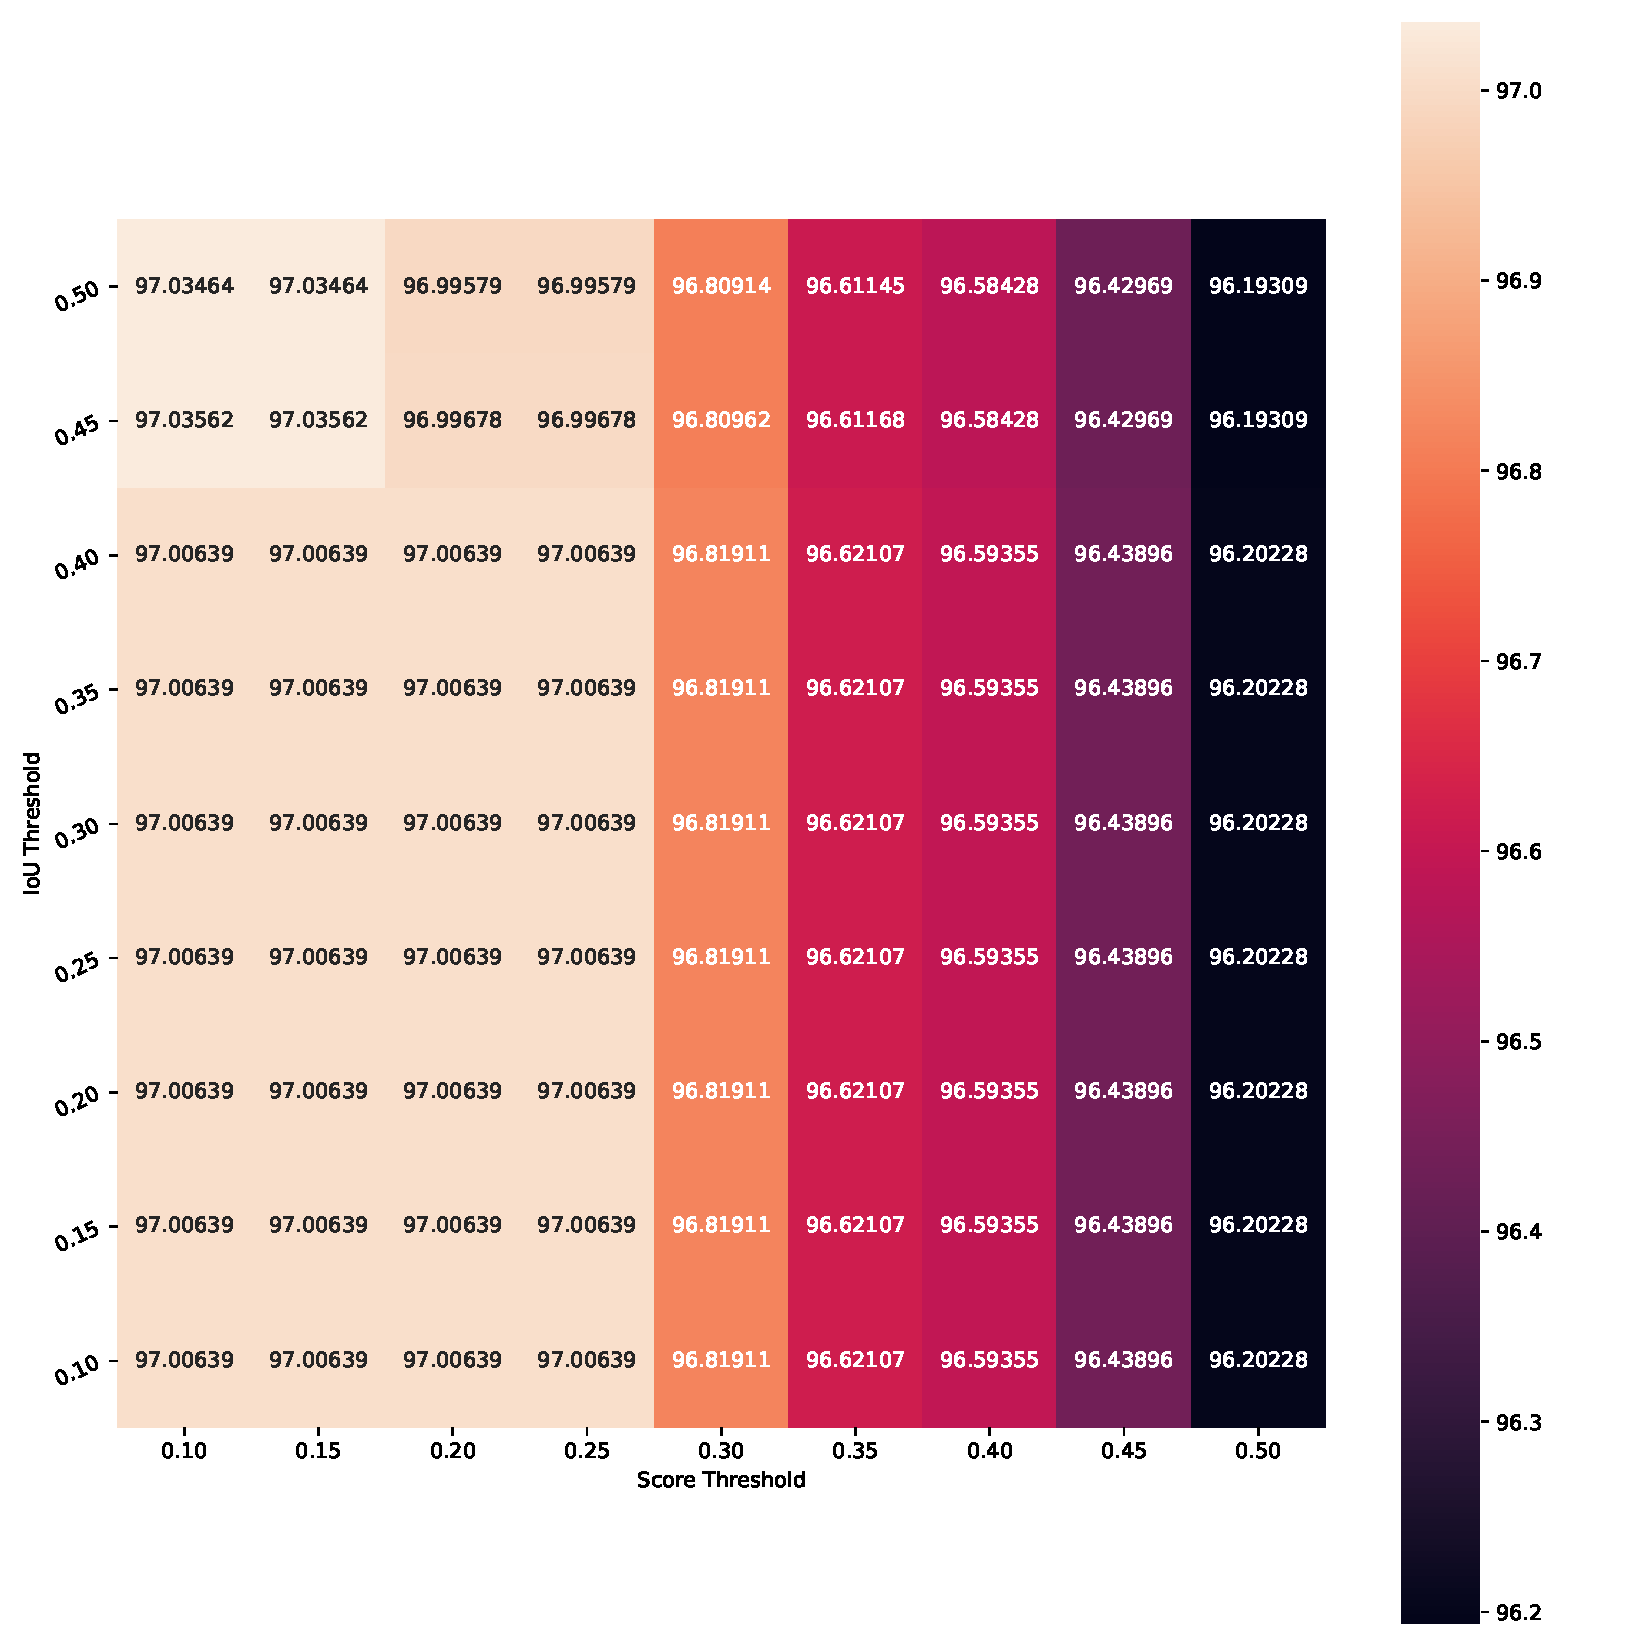
\includegraphics[width=\columnwidth]{imgs/yolo_diou_heat.pdf}
    \caption{The results of the \ac{DIoU}-\ac{NMS} parameter tuning. All possible combinations of score threshold and \ac{IoU} threshold were evaluated on the validation set. The best performing combination is the one with a score threshold of 0.1 and a \ac{IoU} threshold of 0.45.}
    \label{fig:diou_nms_tuning}
\end{center}
\end{figure}

\begin{figure}[H]
\begin{center}
    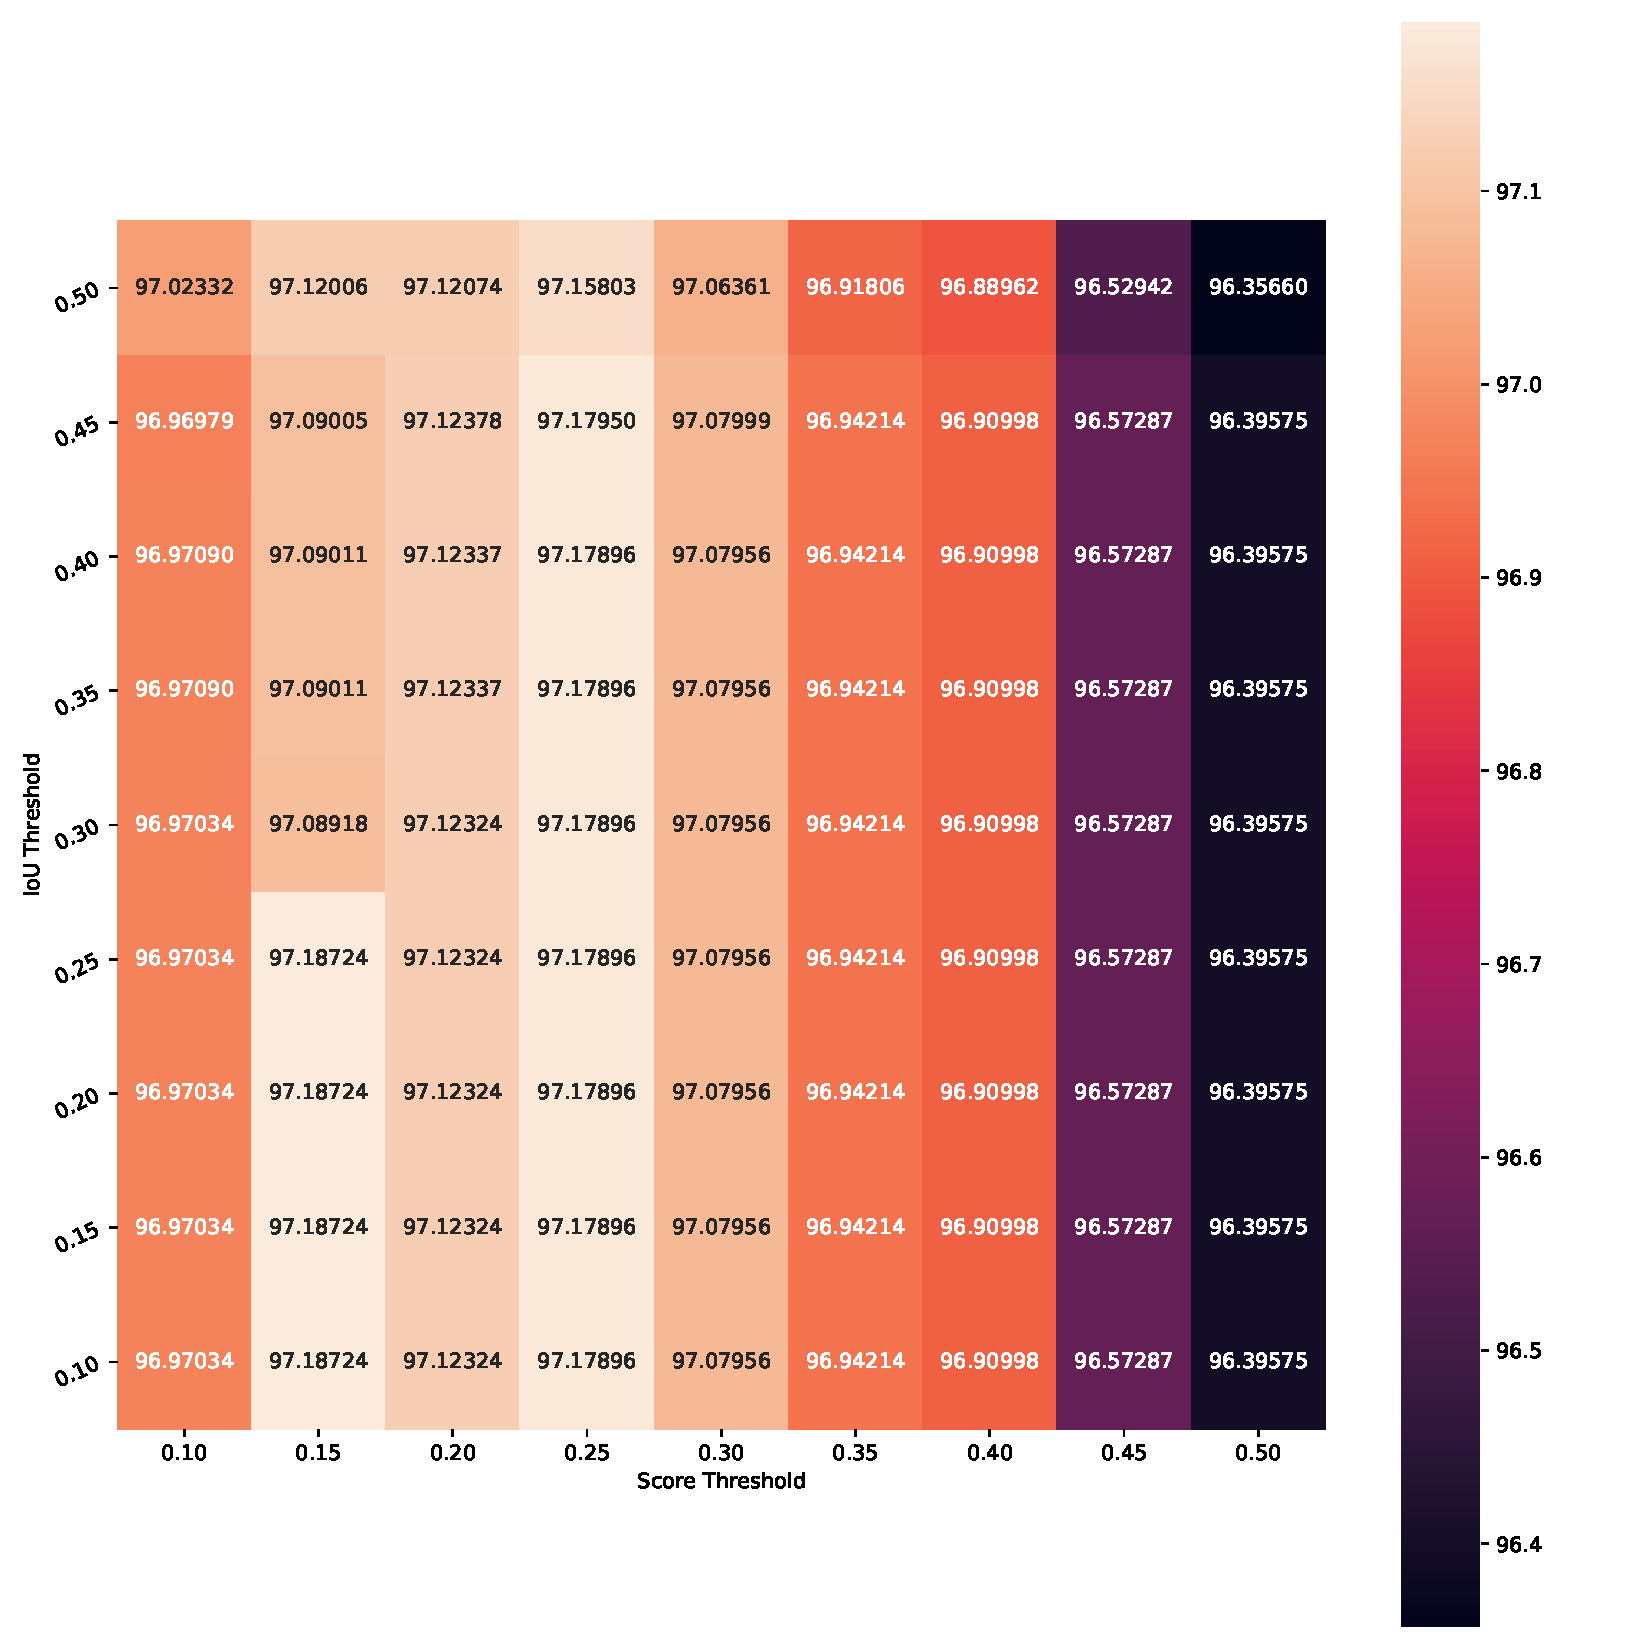
\includegraphics[width=\columnwidth]{imgs/yolo_wbf_heat.pdf}
    \caption{The results of the \ac{WBF} parameter tuning. All possible combinations of score threshold and \ac{IoU} threshold were evaluated on the validation set. The best performing combination is the one with a score threshold of 0.15 and an \ac{IoU} threshold of 0.25.}
    \label{fig:wbf_nms_tuning}
\end{center}
\end{figure}

\begin{figure}[H]
\begin{center}
    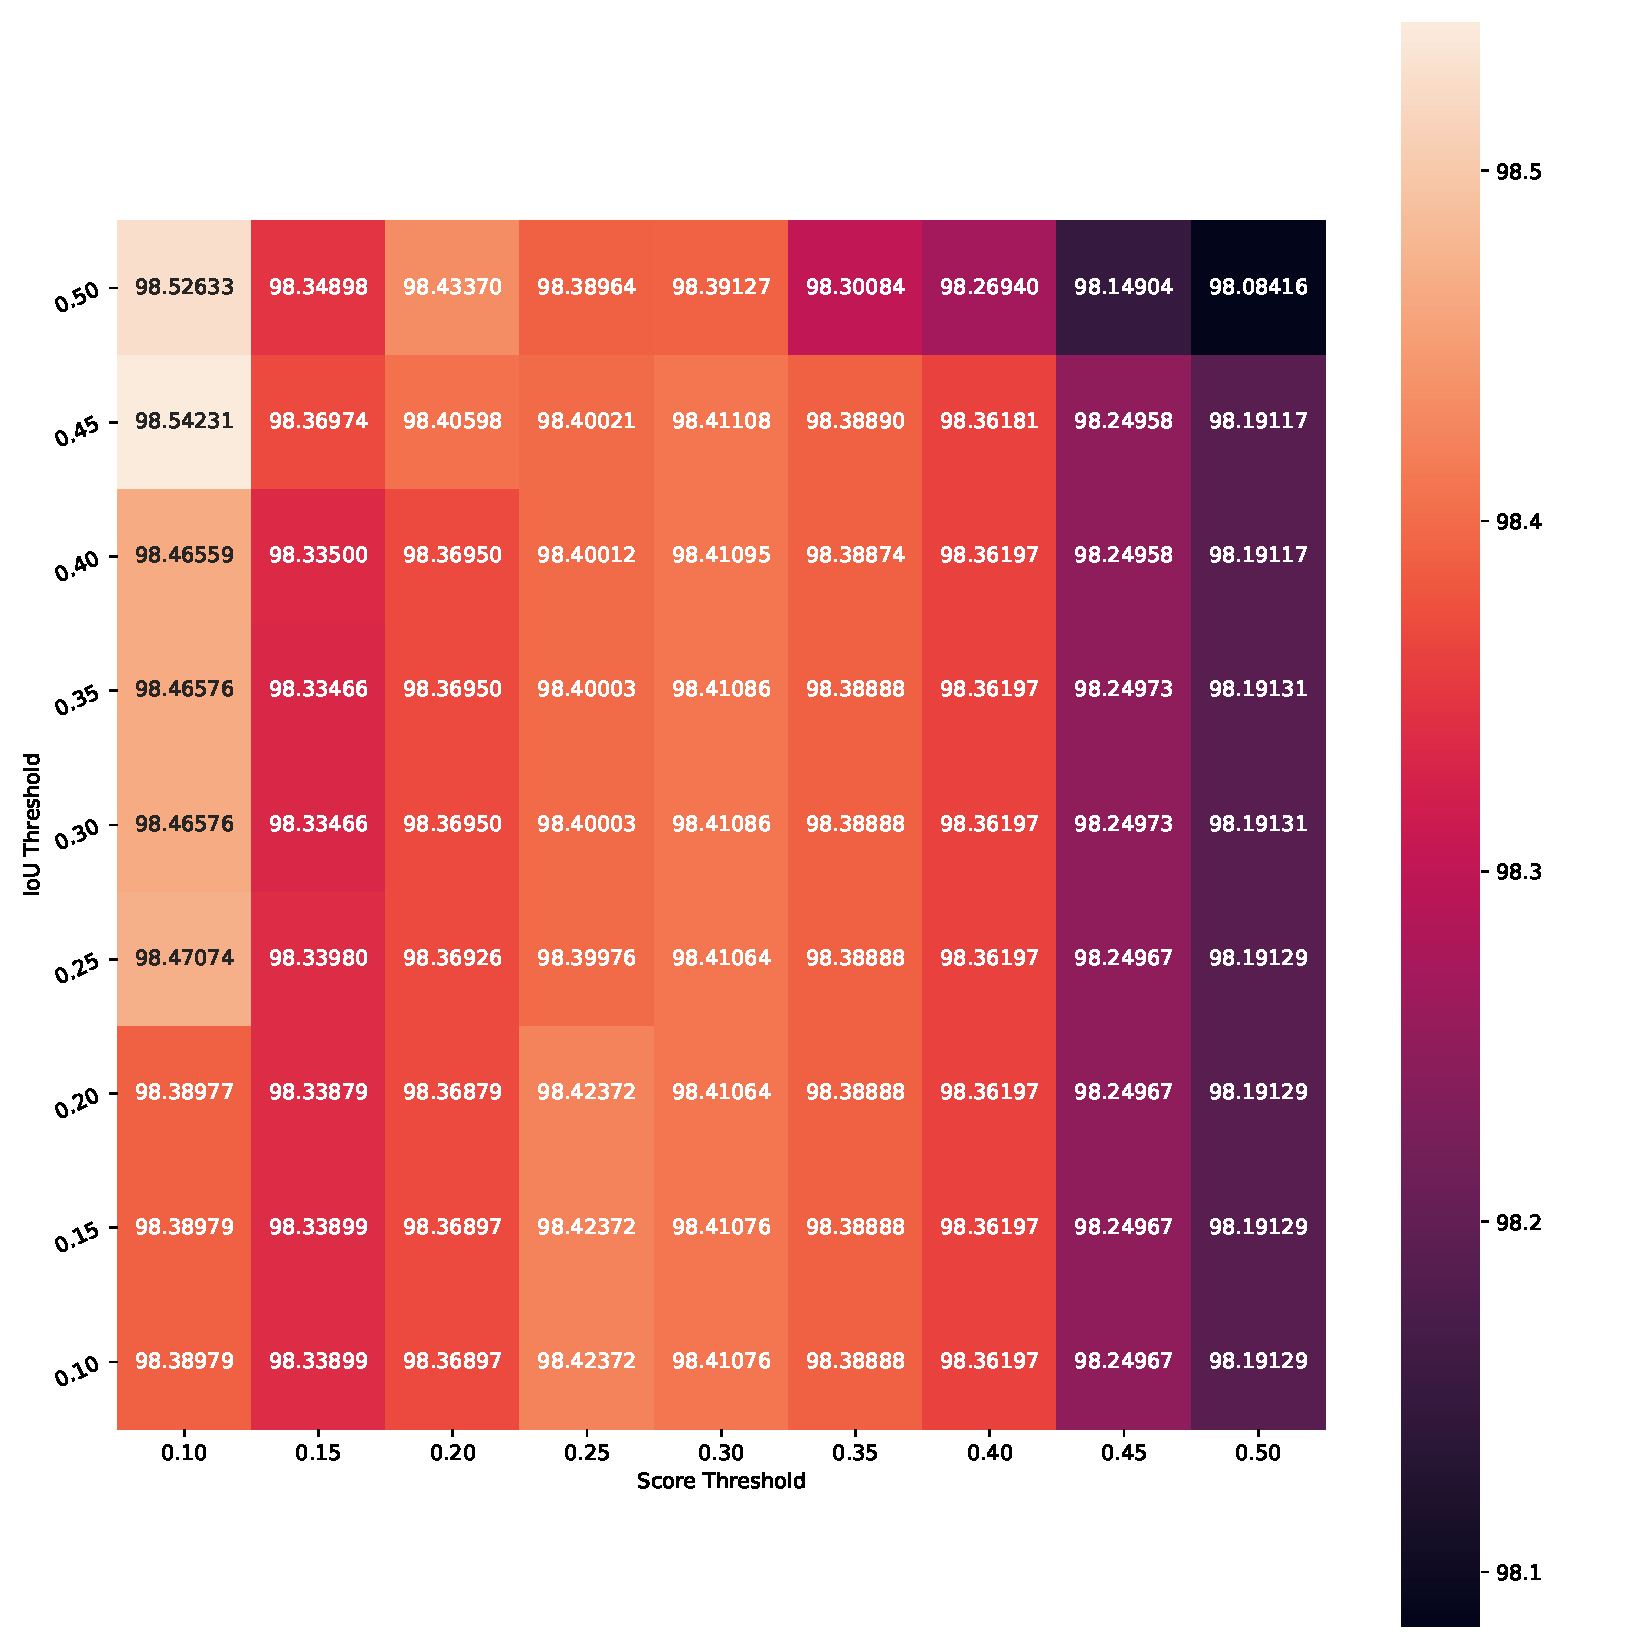
\includegraphics[width=\columnwidth]{imgs/yolo_wbf_tta_heat.pdf}
    \caption{The results of the \ac{WBF} tuning with \ac{TTA}. All possible combinations of score threshold and \ac{IoU} threshold were evaluated on the validation set. The best performing combination is the one with a score threshold of 0.1 and an \ac{IoU} threshold of 0.45.}
    \label{fig:wbf_tta_nms_tuning}
\end{center}
\end{figure}
